
\subsection{ハミルトニアン}

\subsubsection{モデル構築}

昇降演算子$\hat{a},\hat{a}^\dagger$からハミルトニアン$H$を構築する。
ハミルトニアン$H$はエネルギーの次元をもつエルミート演算子である。
昇降演算子$\hat{a},\hat{a}^\dagger$は無次元量であったから、
ハミルトニアンの構築にはエネルギーの次元をもつ定数を導入する必要がある。
量子効果を表すために換算プランク定数$\hbar$を含む必要があるので、
これと組み合わせてエネルギーの次元をもつ定数を構成できるよう
時間の逆数の次元をもつ角振動数$\omega$を導入する。
つまりエネルギーの次元をもつ定数$\hbar\omega$をハミルトニアン$H$の構築に使う。

昇降演算子$\hat{a},\hat{a}^\dagger$で構成される
もっとも一般的な演算子$A$は次の式で書かれる (ansatz)。
\begin{equation}
  \label{eq:A_ansatz}
  A=\sum_{m=0}^\infty\sum_{n=0}^\infty c_{mn}(\hat{a}^\dagger)^m\hat{a}^n
\end{equation}
% textlint-disable
$\hat{a}\hat{a}^\dagger\hat{a}$など他の順序の積をもつ項についても、
交換関係 (\ref{eq:a_algebra}) 式を用いて$\hat{a}^\dagger$を
左に移動させれば (\ref{eq:A_ansatz}) 式と同じ形に帰着させることができる。
% textlint-enable
このうちエルミートとなるものは次の条件を満たす場合。
\begin{equation}
  \label{eq:hermitian_constraint}
  A=A^\dagger
  \Leftrightarrow
  c_{mn} = c^\ast_{nm}
\end{equation}
よって昇降演算子$\hat{a},\hat{a}^\dagger$を用いる
ハミルトニアン$H$の一般形は次の式になる。
\begin{equation}
  \label{eq:H_ansatz}
  H=
  \sum_{m=0}^\infty c_{mm}\hat{N}^m
  +\sum_{m>n\geq0} c_{mn}(\hat{a}^\dagger)^m\hat{a}^n
  +\sum_{n>m\geq0} c^\ast_{nm}(\hat{a}^\dagger)^m\hat{a}^n,\quad
  c_{mm}\in\mathbb{R}
\end{equation}
ただし交換関係 (\ref{eq:a_algebra}) 式を用いたあとに$c_{00}$を再定義した。
系の安定性を考えて固有値に下限をもつハミルトニアンに限ると
一般形はさらに絞り込むことができる。
(\ref{eq:hermitian_constraint})式を用いると$m>n$の場合で次が分かる。
\begin{equation}
  \label{eq:hermitian_decomposite}
  \begin{split}
    &c_{mn}(\hat{a}^\dagger)^m\hat{a}^n
    + c_{nm}(\hat{a}^\dagger)^n\hat{a}^m
    =c_{mn}(\hat{a}^\dagger)^m\hat{a}^n
    + c^\ast_{mn}(\hat{a}^\dagger)^n\hat{a}^m \\
    &=\hat{N}^n
    (c_{mn}(\hat{a}^\dagger)^{m-n}+c^\ast_{mn}\hat{a}^{m-n})
    +\text{const.} \\
    &=\hat{N}^n
    \ab[
      \Re(c_{mn})\ab((\hat{a}^\dagger)^{m-n}+\hat{a}^{m-n})
      +i\Im(c_{mn})\ab((\hat{a}^\dagger)^{m-n}-\hat{a}^{m-n})
    ]+\text{const.}
  \end{split}
\end{equation}
(\ref{eq:H_ansatz})(\ref{eq:hermitian_decomposite})(\ref{eq:xp2a})
式を合わせることで
次を得る。
\begin{equation}
  \begin{split}
    H &= c'_{00} +
    \Re(c_{10})\ab(\hat{a}^\dagger+\hat{a})
    +i\Im(c_{10})\ab(\hat{a}^\dagger-\hat{a})
    +c_{11}\hat{N} \\
    &\quad+\hat{N}
    \ab[
      \Re(c_{20})\ab((\hat{a}^\dagger)^2+\hat{a}^2)
      +i\Im(c_{20})\ab((\hat{a}^\dagger)^2-\hat{a}^2)
    ]
    +\ldots \\
    &= c'_{00} +
    \Re(c_{10})\frac{\sqrt{2}\hat{x}}{L}
    -\Im(c_{10})\frac{\sqrt{2}L\hat{p}}{\hbar}
    +c_{11}\hat{N} \\
    &\quad+\hat{N}
    \ab[\Re(c_{20})
      \ab(
      \frac{\hat{x}^2}{L^2}-\frac{L^2\hat{p}^2}{\hbar^2}
      )
      +\Im(c_{20})
      \frac{1}{\hbar}(\hat{x}\hat{p}+\hat{p}\hat{x})
    ]
    +\ldots
  \end{split}
\end{equation}
ただし定数項を$c_{00}'$に吸収させた。
ここで$\hat{x},\hat{p}$の固有値の値域は
$[-\infty,\infty]$であるから、
$H$からこれらの$-\infty$の固有値を取りうる項を除外するために
次の条件が必要になる。
\begin{equation}
  c_{10}=c_{20}=\ldots=0
\end{equation}
よってハミルトニアン$H$がエルミートで固有値に下限をもつことから
次の一般形を得る。
\begin{equation}
  \hat{H}
  =c'_{00}+c_{11}\hat{N}+\ldots,\quad
  c_{mm}\in\mathbb{R}
\end{equation}
このうち非自明でもっとも簡単なケースは次のケースである。
\begin{equation}
  c'_{11}\neq0,\quad
  c_{mn} = 0\quad(m\geq2\quad\text{or}\quad n\geq2)
\end{equation}
ここで係数$c'_{00},c_{11}$は前述のようにエネルギーの次元をもつように
$\hbar\omega$に比例させるように定義する。
慣例にもとづき比例係数については次のように選ぶ。
\begin{equation}
  \label{eq:ladder_H}
  \hat{H}
  =\frac{\hbar\omega}{2}\ab(\hat{a}^\dagger\hat{a}+\hat{a}\hat{a}^\dagger)
  =\hbar\omega\ab(\hat{a}^\dagger\hat{a}+\frac{1}{2})
  \tag{9.1}
\end{equation}
(\ref{eq:number_op_repr}) 式を用いれば
このハミルトニアン$H$が次の固有値をもつことが分かる。
\begin{equation}
  E_n=\hbar\omega\ab(\omega+\frac{1}{2}),\quad
  n=0,1,2,\ldots
\end{equation}

エネルギースペクトラムの離散性は古典領域$n\gg1$で無視できる。
これはエネルギー準位の相対的な増分が次の式であることから分かる。
\begin{equation}
  \frac{\Delta E}{E} = \frac{1}{n+\frac{1}{2}}
  \overset{n\rightarrow\infty}{\longrightarrow}0
\end{equation}

$\omega$ は現象に応じてさまざまな値をとる。
たとえば共振器オプトメカニクス (Cavity optomechanics) では
レーザ(フォトン)と機械振動(フォノン)の相互作用で量子的な調和振動子を再現する。
観測できる物理量はフォノン側である。
図~\ref{fig:FigureOptomechanicalSystem}に共振オプトメカニクスの概要を示す。
\begin{figure}[tbp]
  \begin{center}
    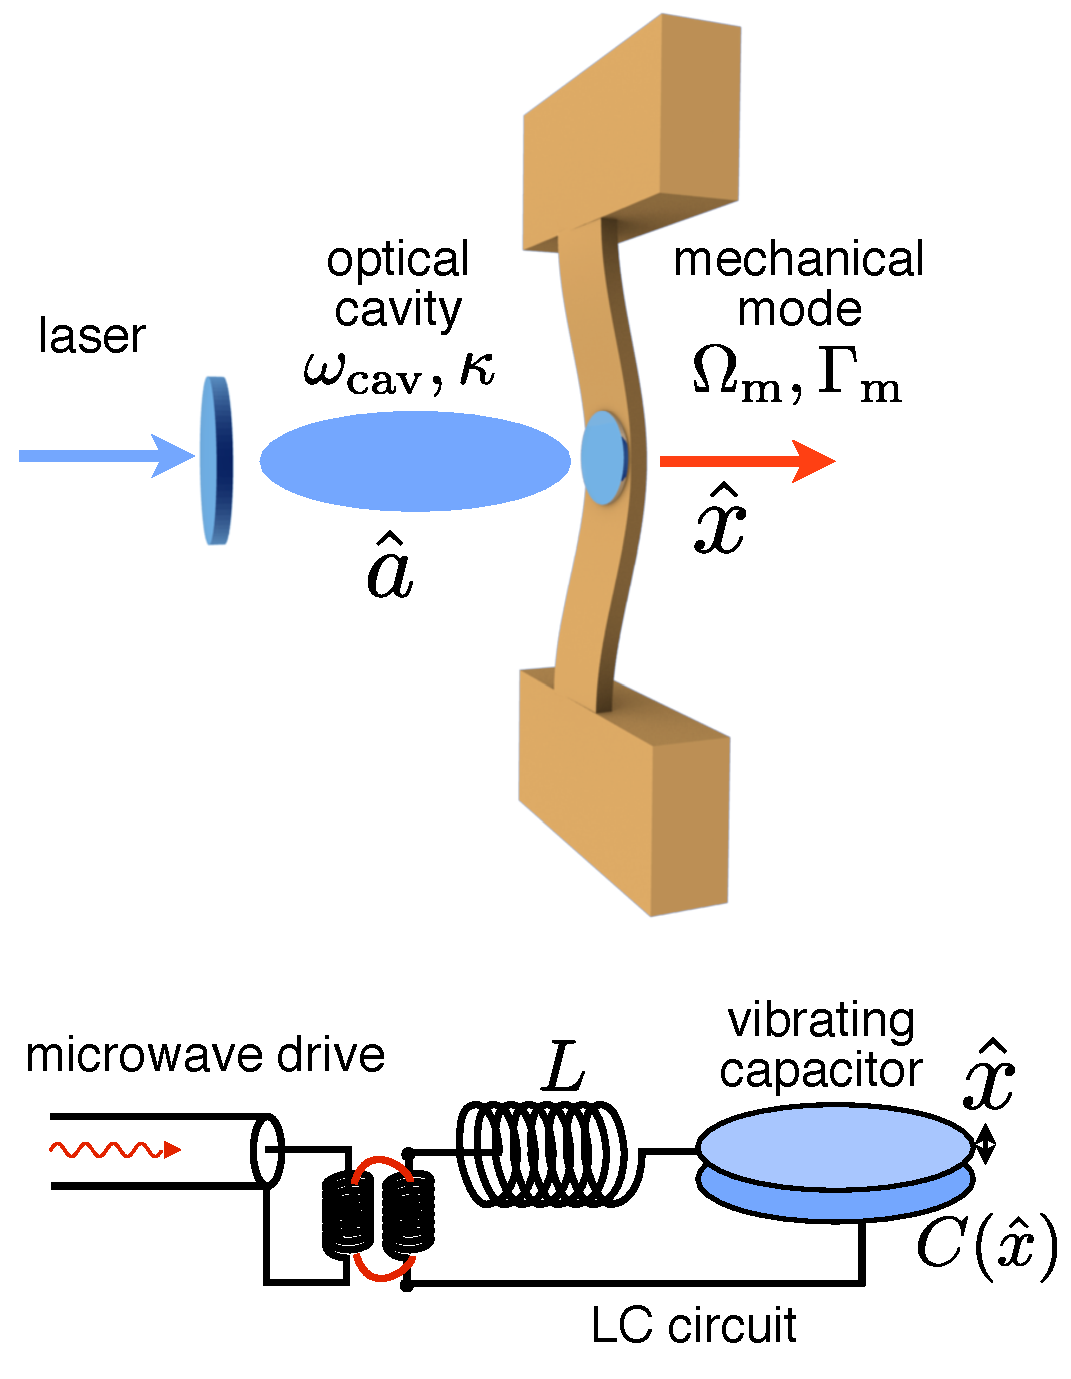
\includegraphics[width=8cm]{img/FigureOptomechanicalSystem.pdf}
    \caption{共振器オプトメカニクスの概要~\cite{aspelmeyer2014cavity}}\label{fig:FigureOptomechanicalSystem}
  \end{center}
\end{figure}
量子的な光共振器 (optical cavity) の物理量を力学現象のモード (mechanical mode) を通じて観測する。
共振器オプトメカニクスの構造をもつ現象は複数知られており、
これまでに実施された実験を図~\ref{fig:Figure_Overview_OptomechanicsFinal}に示す。
\begin{figure}[tbp]
  \begin{center}
    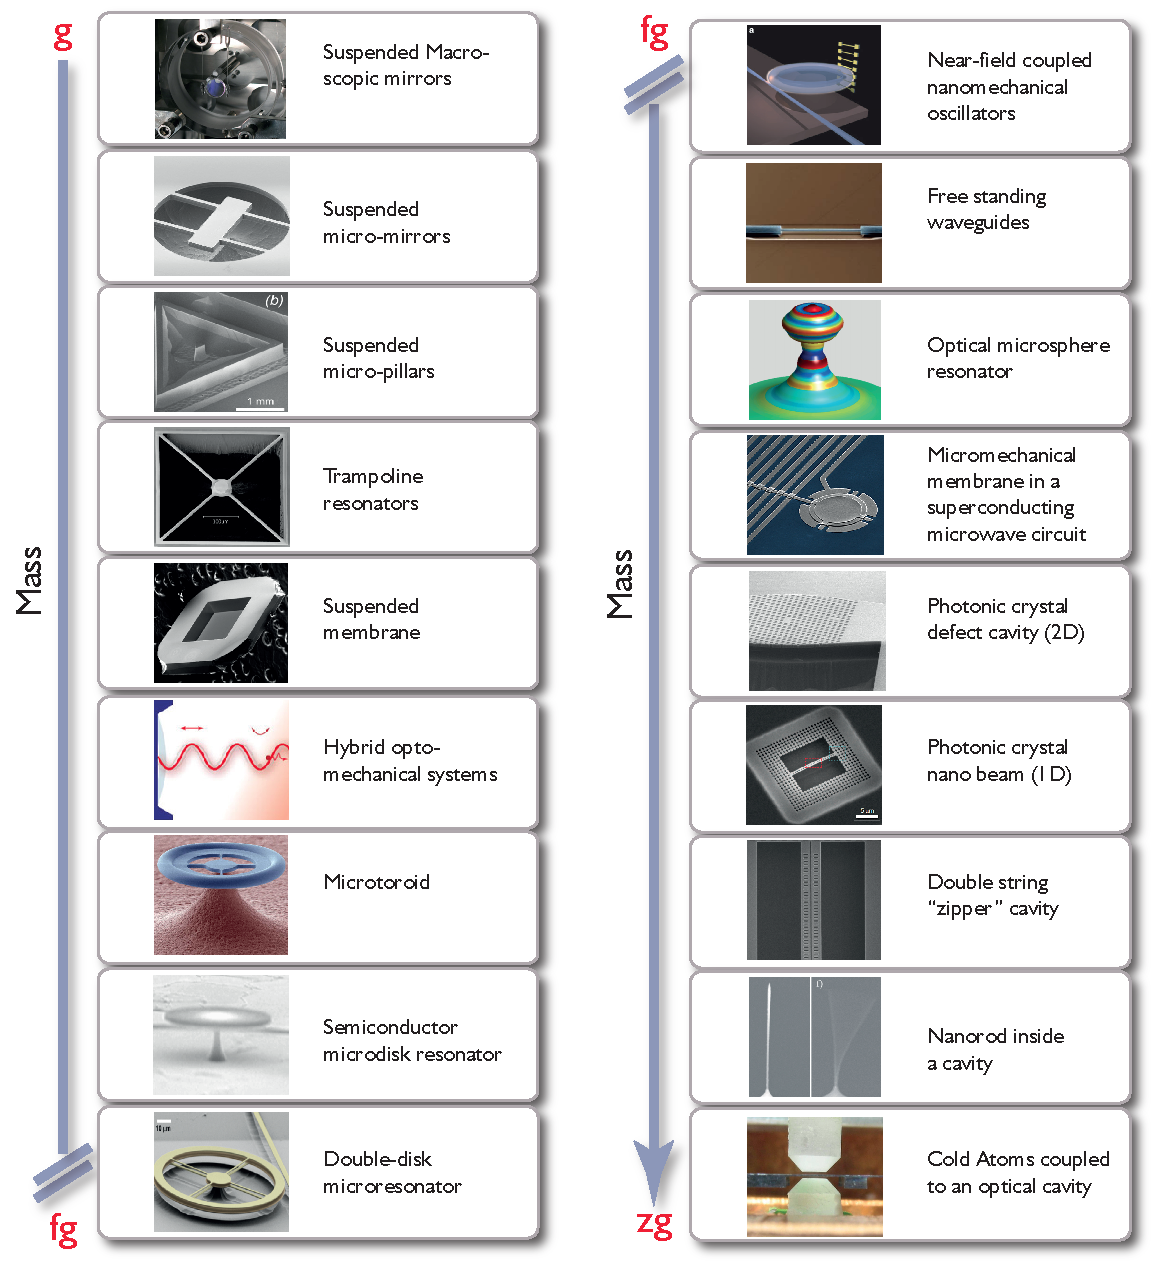
\includegraphics[width=11cm]{img/Figure_Overview_OptomechanicsFinal.png}
    \caption{共振器オプトメカニクスの実験例}\label{fig:Figure_Overview_OptomechanicsFinal}
  \end{center}
\end{figure}
この図では実験に使用されている調和振動子の質量の大きさ$m$でソートされている。
質量単位はフェムトグラム$\si{fg}=10^{-15}\si{g}$がゼプトグラム$\si{zg}=10^{-21}\si{g}$使われている。
共振器オプトメカニクスの実験で観測されている
フォノンの角振動数$\omega$あるいは$\Omega_m$は
図~\ref{fig:cavity_optomechanics_example_table}のとおりである。
\begin{figure}[tbp]
  \begin{center}
    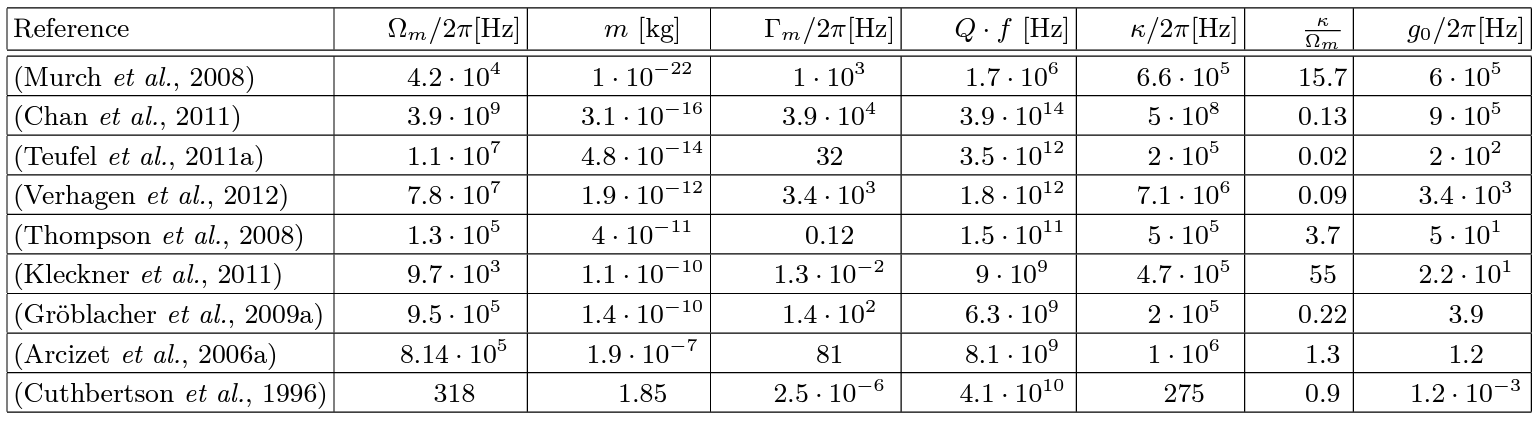
\includegraphics[width=15cm]{img/cavity_optomechanics_example_table.png}
    \caption{共振器オプトメカニクスの実験におけるパラメータ一覧~\cite{aspelmeyer2014cavity}}\label{fig:cavity_optomechanics_example_table}
  \end{center}
\end{figure}
角振動数$\omega$の取りうる単位はおおむね$10^2\sim10^9\si{Hz}$のオーダーである。
この場合$\hbar\omega$の値は$10^{-14}\sim10^{-7}\si{eV}$ほどになる。
$1\si{eV}$は電子1個が$1\si{V}$の電位差から得る位置エネルギーを指す。
また図~\ref{fig:cavity_optomechanics_example_table}から系の特徴的な長さ$L$が次の式で計算可能である。
\begin{equation}
  \label{eq:L_estimate}
  L=\sqrt{\frac{\hbar}{m\omega}}
  \tag{9.3}
\end{equation}
この式で特徴的長さ$L$が見積もれることは次の次元解析から分かる。
\begin{equation}
  [\hbar\omega]=[E]=[mc^2]=ML^2T^{-2}
  \Rightarrow
  \ab[\frac{\hbar}{m\omega}]
  =\ab[\frac{\hbar\omega}{m\omega^2}]
  = ML^2T^{-2}(MT^{-2})^{-1}=L^2
\end{equation}
図~\ref{fig:cavity_optomechanics_example_table}のケースでは
特徴的長さ$L$は$1\si{am}\sim1\si{nm}$程である。

昇降演算子によるハミルトニアン (\ref{eq:ladder_H}) 式の
位置・運動量演算子$\hat{x},\hat{p}$による表示を得るには
(\ref{eq:a2xp})式を用いて次のように変形すればよい。
\begin{equation}
  \begin{split}
    \hat{H}
    &=\hbar\omega\ab(\hat{a}^\dagger\hat{a}+\frac{1}{2})
    =\hbar\omega\ab[
      \frac{1}{\sqrt{2}}
      \ab(\frac{\hat{x}}{L}-i\frac{L\hat{p}}{\hbar})
      \cdot
      \frac{1}{\sqrt{2}}
      \ab(\frac{\hat{x}}{L}+i\frac{L\hat{p}}{\hbar})
      +\frac{1}{2}
    ] \\
    &=\frac{\hbar\omega}{2}\ab[
      \frac{\hat{x}^2}{L^2}
      -\frac{1}{i\hbar}(\hat{x}\hat{p}-\hat{p}\hat{x})
      +\frac{L^2\hat{p}^2}{\hbar^2}
      +1
    ] \\
    &=\frac{\hbar\omega}{2}\ab[
      \frac{\hat{x}^2}{L^2}
      +\frac{L^2\hat{p}^2}{\hbar^2}
    ]
  \end{split}
\end{equation}
ただし位置・運動量演算子$\hat{x},\hat{p}$の交換関係 (\ref{eq:xp_alg}) 式を用いた。
特徴的長さ$L$の推定 (\ref{eq:L_estimate}) 式を代入すると次の結果を得る。
\begin{equation}
  \label{eq:H_xp}
  \hat{H}=\frac{1}{2m}\hat{p}^2+\frac{m\omega^2}{2}\hat{x}^2
  \tag{9.4}
\end{equation}
実際には$L$の式は推定に過ぎないので$\mathcal{O}(1)$の不定性があるが、
$m,\omega$の再定義や単位系の取り直しで吸収したこととする。

\subsubsection{ハミルトニアンから定まる時間発展}

位置・運動量に関するハイゼンベルグ演算子は次の式で定義される。
\begin{equation}
  \begin{split}
    \hat{x}_H
    &=\exp\ab(\frac{it}{\hbar}\hat{H})\hat{x}\exp\ab(-\frac{it}{\hbar}\hat{H}), \\
    \hat{p}_H
    &=\exp\ab(\frac{it}{\hbar}\hat{H})\hat{p}\exp\ab(-\frac{it}{\hbar}\hat{H})
  \end{split}
  \tag{9.5}
\end{equation}
これらの時間発展はハミルトニアン$\hat{H}$による
ハイゼンベルグ方程式 (\ref{eq:heisenberg_eq}) 式から求まる。
位置演算子$\hat{x}_H(t)$の時間発展は次のとおりである。
\begin{equation}
  \begin{split}
    &\odv{}{t}\hat{x}_H(t)
    =\frac{1}{i\hbar}\ab[\hat{x}_H(t),\hat{H}]
    =\frac{1}{i\hbar}
    \ab[
      \exp\ab(\frac{it}{\hbar}\hat{H})
      \hat{x}
      \exp\ab(-\frac{it}{\hbar}\hat{H}),
      \hat{H}
    ] \\
    &=\frac{1}{i\hbar}
    \exp\ab(\frac{it}{\hbar}\hat{H})
    \ab[\hat{x},\hat{H}]
    \exp\ab(-\frac{it}{\hbar}\hat{H})
    \\
    &=\frac{1}{i\hbar}
    \exp\ab(\frac{it}{\hbar}\hat{H})
    \ab[
      \hat{x},\frac{1}{2m}\hat{p}^2+\frac{m\omega^2}{2}\hat{x}^2
    ]
    \exp\ab(-\frac{it}{\hbar}\hat{H})
    \\
    &=\frac{1}{i\hbar}
    \exp\ab(\frac{it}{\hbar}\hat{H})
    \frac{1}{2m}
    \ab(\ab[\hat{x},\hat{p}]\hat{p}+\hat{p}\ab[\hat{x},\hat{p}])
    \exp\ab(-\frac{it}{\hbar}\hat{H})\\
    &=\frac{1}{m}\hat{p}_H(t)
  \end{split}
\end{equation}
運動量演算子$\hat{p}_H(t)$の時間発展は次のとおりである。
\begin{equation}
  \begin{split}
    &\odv{}{t}\hat{p}_H(t)
    =\frac{1}{i\hbar}\ab[\hat{p}_H(t),\hat{H}]
    =\frac{1}{i\hbar}
    \ab[
      \exp\ab(\frac{it}{\hbar}\hat{H})
      \hat{p}
      \exp\ab(-\frac{it}{\hbar}\hat{H}),
      \hat{H}
    ] \\
    &=\frac{1}{i\hbar}
    \exp\ab(\frac{it}{\hbar}\hat{H})
    \ab[\hat{p},\hat{H}]
    \exp\ab(-\frac{it}{\hbar}\hat{H})
    \\
    &=\frac{1}{i\hbar}
    \exp\ab(\frac{it}{\hbar}\hat{H})
    \ab[
      \hat{p},\frac{1}{2m}\hat{p}^2+\frac{m\omega^2}{2}\hat{x}^2
    ]
    \exp\ab(-\frac{it}{\hbar}\hat{H})
    \\
    &=\frac{1}{i\hbar}
    \exp\ab(\frac{it}{\hbar}\hat{H})
    \frac{m\omega^2}{2}
    \ab(\ab[\hat{p},\hat{x}]\hat{p}+\hat{p}\ab[\hat{p},\hat{x}])
    \exp\ab(-\frac{it}{\hbar}\hat{H})\\
    &=-m\omega^2\hat{x}_H(t)
  \end{split}
\end{equation}
結果をまとめると次のとおりである。
\begin{equation}
  \begin{split}
    &\odv{}{t}\hat{x}_H(t)=\frac{1}{m}\hat{p}_H(t), \\
    &\odv{}{t}\hat{p}_H(t)=-m\omega^2\hat{x}_H(t)
  \end{split}
  \tag{9.6}
\end{equation}
この式は古典論の調和振動子の正準方程式と対応している。
これは古典論ではハミルトニアンがポアソン括弧における時間発展の生成子になっていることと、
ハイゼンベルク方程式に対応があることからも分かる。
よって (\ref{eq:H_xp}) 式は量子的な調和振動子のハミルトニアンであることが直感的に分かる。

(\ref{eq:H_xp}) 式のハミルトニアンを構成する際に、
昇降演算子$\hat{a}^\dagger,\hat{a}$の高次項を0とした。
(\ref{eq:a2xp}) 式を用いると$\hat{x},\hat{p}$の高次項を0としたことが分かる。
これは非線形相互作用を線形化あるいは無視した状況に対応する。
このようなハミルトニアン$\hat{H}$は線形応答を解析する際に現れる。

\subsubsection{零点エネルギーとカシミール効果}

基底状態はエネルギー0ではなく次の零点エネルギー (zero-point energy) をもつ。
\begin{equation}
  \hat{H}\ket{0} = \frac{1}{2}\hbar\omega\ket{0}
\end{equation}
零点エネルギーが生じる理由は$\Delta x,\Delta p$ に関する次のケナード不等式によるものである。
\begin{equation}
  \Delta x \Delta p\geq\frac{\hbar}{2}
\end{equation}
ハミルトニアン$H$に対する固有値であるエネルギー準位の下限は
ケナード不等式の下限$\Delta x\Delta p=\dfrac{\hbar}{2}$で評価できる。
(\ref{eq:H_xp}) 式の各項の不確定性を考えることで次のように評価できる。
\begin{equation}
  E(\Delta x)
  =\frac{1}{2m}\Delta p^2+\frac{m\omega^2}{2}\Delta x^2
  \geq2\sqrt{\frac{1}{2m}\Delta p^2\cdot\frac{m\omega^2}{2}\Delta x^2}
  =\frac{1}{2}\hbar\omega
\end{equation}
ただし相加平均・相乗平均の関係式を用いた。
等号成立条件は次の式である。
\begin{equation}
  \frac{m\omega^2}{2}\Delta x^2
  =\frac{1}{2m}\Delta p^2
  =\frac{1}{2m}\ab(\frac{\hbar}{2\Delta x})^2
  \Leftrightarrow
  \Delta x^4 = \frac{\hbar^2}{4m^2\omega^2}
  \Leftrightarrow
  \Delta x = \sqrt{\frac{\hbar}{2m\omega}}
  \tag{9.18}
\end{equation}
これは零点エネルギーそのものである。

零点エネルギーはカシミール効果などを通じて物理的意味をもつケースがある。
カシミール効果は金属場の間に生じる零点エネルギーによって力が働く現象を指す。
カシミール効果は電磁場に対する場の量子論で計算できる。
ここでは簡単に説明するために電磁場が偏光で2自由度あること~\cite{mio2012em}と、
自由スカラー場の量子化が無限個の調和振動子の集まりと等価であること~\cite{watamura2024qft}を利用する。
上記の事実を使うと相対論的量子力学の自由電磁場に対するハミルトニアンは次の構造をもつことが分かる。
\begin{equation}
  \hat{H}
  \propto
  \sum_{\lambda=0,1}
  \int\d^3p\,\hbar\omega_{\vec{p}}\,
  \ab[
    \ab(a^{(\lambda)}_{\vec{p}})^\dagger a^{(\lambda)}_{\vec{p}}
    +\frac{1}{2}
  ]
\end{equation}
非積分関数は偏光$\lambda$で運動量$\vec{p}$の光子のもつハミルトニアン密度を指す。
真空$\ket{0}$では光子が存在しないので次の式を満たす。
\begin{equation}
  \forall \lambda\in{0,1},\quad
  \forall \vec{p}\in\mathbb{R}^3,\quad
  \ab(a^{(\lambda)}_{\vec{p}})^\dagger a^{(\lambda)}_{\vec{p}}\ket{0}=0
\end{equation}
よって真空のエネルギー期待値は次の式になる。
\begin{equation}
  \braket{0|\hat{H}|0}
  \propto
  \int\d^3p\,\hbar\omega_{\vec{p}}
\end{equation}
特殊相対性理論では質量$m$、運動量$\vec{p}$、エネルギー$E_{\vec{p}}$には
次の関係がある。
\begin{equation}
  E_{\vec{p}}^2=m^2c^4+\vec{p}^2c^2
\end{equation}
ただし$c$は光速である。
光子の質量$m$は0あり、
運動量$\vec{p}$の光子1つあたりのエネルギーが$E_{\vec{p}}=\hbar\omega_{\vec{p}}$であるので
次の式が成り立つ。
\begin{equation}
  \hbar\omega_{\vec{p}}=c|\vec{p}|
\end{equation}
$z$軸方向に幅$d$で平行に金属板を配置すると
金属板上で電磁場が0となるよう次のように波のモードが制限される。
\begin{equation}
  p_z=\frac{n\pi}{d}
  \Rightarrow
  \hbar\omega^{(n)}_{\vec{p}}
  = c\sqrt{p_x^2+p_y^2+\frac{n^2\pi^2}{d^2}},\quad
  n\in\mathbb{Z}
\end{equation}
これよりハミルトニアン$H$の$p_z$方向の積分も次のように離散化される。
\begin{equation}
  \braket{0|\hat{H}_d|0}
  \propto
  \sum_{n=1}^\infty
  \int\d p_x\d p_y\,\hbar\omega^{(n)}_{\vec{p}}
\end{equation}
ただし離散化後のハミルトニアンを $\hat{H}_d$ と書いた。
以下で真空のエネルギーの期待値を極座標系への変数変換を用いて評価する。
\begin{equation}
  \begin{split}
    \braket{0|\hat{H}_d|0}
    &\propto\sum_{n=1}^\infty
    \int\d p_x\d p_y\,\sqrt{p_x^2+p_y^2+\frac{n^2\pi^2}{d^2}} \\
    &=\sum_{n=1}^\infty
    \int_0^\infty\d p\int_0^{2\pi}\d \theta\,p\sqrt{p^2+\frac{n^2\pi^2}{d^2}} \\
    &\propto
    \sum_{n=1}^\infty
    \int_0^\infty\d p\,p\sqrt{p^2+\frac{n^2\pi^2}{d^2}}
  \end{split}
\end{equation}
ここで簡単のために$C_n^2\equiv\dfrac{n^2\pi^2}{d^2}$とし、
$p^2\equiv C_n^2\tan^2\theta$と変数変換すると次のように評価可能である。
\begin{equation}
  \begin{split}
    &\int_0^\infty\d p\,p\sqrt{p^2+C_n^2}
    \propto\int_0^\infty\d (p^2)\sqrt{p^2+C_n^2}
    \propto\int_0^{\pi/2}
    \frac{C_n^2\tan\theta}{\cos^2\theta}
    \d\theta\,
    C_n\sqrt{1+\tan^2\theta} \\
    &=C_n^3\int_0^{\pi/2}
    \frac{\tan\theta}{\cos^2\theta}
    \d\theta\,
    \frac{1}{|\cos\theta|}
    =C_n^3\int_0^{\pi/2}
    \ab(\sin\theta\d\theta)\,
    \cos^{-4}\theta
    =C_n^3\int_0^1
    \d\ab(\cos\theta)\,
    \cos^{-4}\theta \\
    &=C_n^3\ab[-\frac{1}{3}\cos^{-3}\theta]_{\cos\theta=0}^{\cos\theta=1}
    \propto-\ab(\frac{n\pi}{d})^3
  \end{split}
\end{equation}
したがって正則化された真空エネルギーの期待値はゼータ関数$\zeta(n)$を用いて次のように書ける。
\begin{equation}
  \braket{0|\hat{H}_d|0}
  \propto
  -\sum_{n=1}^\infty\ab(\frac{n\pi}{d})^3
  \propto-d^{-3}\sum_{n=1}^\infty n^3
  =-d^{-3}\zeta(-3)
\end{equation}
ただし次のゼータ関数$\zeta(s)$の定義を用いた。
\begin{equation}
  \label{eq:zeta_positive}
  \begin{split}
    \zeta(s)
    \equiv\sum_{n=1}^\infty n^{-s}
  \end{split}
\end{equation}
(\ref{eq:zeta_positive})式ではゼータ関数$\zeta(s)$は$s\in\mathbb{R}_+$のみで収束する。
一方で解析接続を用いて定義域を拡大し$s\in\mathbb{C}$で定義しなおせば$\zeta(-3)$は有限の値で評価できる。
\begin{equation}
  \label{eq:zeta_reg}
  \zeta(-3)=\frac{1}{120}
  \Rightarrow
  \braket{0|\hat{H}|0}\propto -d^{-3}
\end{equation}
このように解析接続で定義されたゼータ関数$\zeta(s)$を用いて
物理量を有限の値で評価することをゼータ関数正則化と呼ぶ。

この結果は次のカットオフ$\epsilon\sim0$による正則化からも評価できる。
\begin{equation}
  \begin{split}
    &\zeta_\epsilon(-3)
    \equiv
    \sum_{n=1}^\infty n^3e^{-n\epsilon}
    =-\odv[order=3]{}{\epsilon} \sum_{n=1}^\infty e^{-n\epsilon}
    =-\odv[order=3]{}{\epsilon} \frac{e^{-\epsilon}}{1-e^{-\epsilon}}
    =\odv[order=3]{}{\epsilon} \frac{1}{1-e^\epsilon} \\
    &=\odv[order=2]{}{\epsilon} \frac{e^\epsilon}{(1-e^\epsilon)^2}
    =\odv{}{\epsilon}\ab(
    \frac{e^\epsilon}{(1-e^\epsilon)^2}
    +\frac{2e^{2\epsilon}}{(1-e^\epsilon)^3}
    )
    =\frac{e^\epsilon}{(1-e^\epsilon)^2}
    +\frac{2e^{2\epsilon}}{(1-e^\epsilon)^3}
    +\frac{4e^{2\epsilon}}{(1-e^\epsilon)^3}
    +\frac{6e^{3\epsilon}}{(1-e^\epsilon)^4} \\
    &=\frac{1}{(1-e^\epsilon)^4}
    \ab[e^\epsilon(1-e^\epsilon)^2+6e^{2\epsilon}(1-e^\epsilon)+6e^{3\epsilon}]
    =\frac{1}{(1-e^\epsilon)^4}
    \ab(e^\epsilon+4e^{2\epsilon}+e^{3\epsilon}) \\
    &=\ab(
    -\epsilon-\frac{1}{2}\epsilon^2-\frac{1}{6}\epsilon^3
    -\frac{1}{24}\epsilon^4-\frac{1}{120}\epsilon^5+\mathcal{O}(\epsilon^6)
    )^{-4} \\
    &\qquad\times\left[
      \ab(1+\epsilon+\frac{1}{2}\epsilon^2+\frac{1}{6}\epsilon^3+\frac{1}{24}\epsilon^4)
      +4\ab(1+2\epsilon+2\epsilon^2+\frac{4}{3}\epsilon^3+\frac{2}{3}\epsilon^4)\right. \\
      &\qquad\qquad\left.
      +\ab(1+3\epsilon+\frac{9}{2}\epsilon^2+\frac{9}{2}\epsilon^3+\frac{27}{8}\epsilon^4)
      +\mathcal{O}(\epsilon^5)
      \right] \\
    &=\epsilon^{-4}\frac{1}{
      (1+\frac{1}{2}\epsilon+\frac{1}{6}\epsilon^2+\frac{1}{24}\epsilon^3
      +\frac{1}{120}\epsilon^4+\mathcal{O}(\epsilon^5))^4}
    \ab(
    6+12\epsilon+13\epsilon^2+10\epsilon^3+\frac{73}{12}\epsilon^4
    +\mathcal{O}(\epsilon^5)
    )
  \end{split}
\end{equation}
ここで次のマクローリン展開を利用する。
\begin{equation}
  (1+x)^{-4}
  =1-4x+10x^2-20x^3+35x^4+\mathcal{O}(x^5)
\end{equation}
このとき次の級数展開が可能。
\begin{equation}
  \begin{split}
    &\ab(1+\frac{1}{2}\epsilon+\frac{1}{6}\epsilon^2+\frac{1}{24}\epsilon^3
    +\frac{1}{120}\epsilon^4)^{-4} \\
    &=1-4\ab(\frac{1}{2}\epsilon+\frac{1}{6}\epsilon^2+
    \frac{1}{24}\epsilon^3+\frac{1}{120}\epsilon^4)
    +10\ab(\frac{1}{2}\epsilon+\frac{1}{6}\epsilon^2+\frac{1}{24}\epsilon^3)^2 \\
    &\qquad
    -20\ab(\frac{1}{2}\epsilon+\frac{1}{6}\epsilon^2)^3
    +35\ab(\frac{1}{2}\epsilon)^4
    +\mathcal{O}(\epsilon^5) \\
    &=1-2\epsilon+\frac{11}{6}\epsilon^2-\epsilon^3+\frac{251}{720}\epsilon^4
    +\mathcal{O}(\epsilon^5)
  \end{split}
\end{equation}
よって$\zeta(-3)$の正則化$\zeta_\epsilon(-3)$は次の式になる。
\begin{equation}
  \begin{split}
    &\zeta_\epsilon(-3)
    =\epsilon^{-4}
    \ab(1-2\epsilon+\frac{11}{6}\epsilon^2-\epsilon^3
    +\frac{251}{720}\epsilon^4+\mathcal{O}(\epsilon^5))
    \ab(
    6+12\epsilon+13\epsilon^2+10\epsilon^3+\frac{73}{12}\epsilon^4
    +\mathcal{O}(\epsilon^5)
    ) \\
    &=\epsilon^{-4}\ab(6+\frac{1}{120}\epsilon^4+\mathcal{O}(\epsilon^5)) \\
    &=\frac{6}{\epsilon^4}+\frac{1}{120}+\mathcal{O}(\epsilon)
  \end{split}
\end{equation}

ここで$\epsilon\rightarrow0$とする前に真空エネルギーの期待値を評価する。
$e^{-n\epsilon}$の効果は$\zeta(-3)$の級数のうち
$n>\dfrac{1}{\epsilon}$の項の効果を抑制する。
これは真空エネルギーの期待値$\braket{0|\hat{H}|0}$における
モードを$p_z<\dfrac{\pi}{\epsilon d}$に制限することと同じである。
これは高エネルギーのモードを制限している(UV 正則化)。
そこでこの上限のモードを$p_z^c$と書いて定義する。
\begin{equation}
  p_z^c\equiv\frac{\pi}{\epsilon d}
  \Rightarrow
  \frac{1}{\epsilon}\propto p_z^c d
\end{equation}
よって$\epsilon\rightarrow0$はエネルギー上限を無制限にする極限
$p_z^c\rightarrow\infty$と等価である。
このとき次の式で評価できる。
\begin{equation}
  \begin{split}
    &\braket{0|\hat{H}_d|0}
    \propto
    -d^{-3}\zeta(-3)
    =\lim_{p_z^c\rightarrow\infty}
    \ab[-d^{-3}\ab(
    C(p_z^cd)^4
    +\frac{1}{120}
    +\mathcal{O}\ab(\frac{1}{p_z^c d})
    )] \\
    &=\lim_{p_z^c\rightarrow\infty}\ab[
      -C(p_z^c)^4d-\frac{1}{120d^3}+\mathcal{O}\ab(\frac{1}{p_z^cd^4})]
  \end{split}
\end{equation}
ただし$C$は$\mathcal{O}(1)$の定数である。
実際には真空エネルギーの期待値の計算は金属板外のハミルトニアンも加えて計算する必要がある。
金属板外のハミルトニアンは$\hat{H}_\infty$だが、
発散の度合いを評価するため
$\lim_{L\rightarrow\infty}\hat{H}_{L-d}$とする。
これは宇宙の大きさを制限している(IR 正則化)。
このとき合計の真空エネルギーの期待値は次のとおりである。
\begin{equation}
  \begin{split}
    &\braket{0|\hat{H}_d|0}+\braket{0|\hat{H}_\infty|0}
    =\lim_{L\rightarrow\infty}\ab(\braket{0|\hat{H}_d|0}+\braket{0|\hat{H}_{L-d}|0}) \\
    &\propto\lim_{p_z^c\rightarrow\infty}\lim_{L\rightarrow\infty}
    \ab(-C(p_z^c)^4L
    +\frac{1}{120d^3}-\frac{1}{120(L-d)^3}
    +\mathcal{O}\ab(\frac{1}{p_z^cd^4})+\mathcal{O}\ab(\frac{1}{p_z^c(L-d)^4}))
  \end{split}
\end{equation}
よって真空エネルギーの期待値に起因する力はこの微分で与えられるから、
次の式で評価できる。
\begin{equation}
  \begin{split}
    &\odv{}{d}\ab(\braket{0|\hat{H}_d|0}+\braket{0|\hat{H}_\infty|0}) \\
    &\propto\lim_{p_z^c\rightarrow\infty}\lim_{L\rightarrow\infty}
    \ab(
    \frac{1}{40d^4}+\frac{1}{40(L-d)^4}
    +\mathcal{O}\ab(\frac{1}{p_z^cd^5})+\mathcal{O}\ab(\frac{1}{p_z^c(L-d)^5})) \\
    &=\frac{1}{40d^4}
  \end{split}
\end{equation}
この結果は (\ref{eq:zeta_reg}) 式による結果と同一である。
つまりゼータ関数正則化は解析接続によるゼータ関数の再定義を通じて、
UV・IR 正則化と同等の働きをしていたことが分かる。